\documentclass[tikz, border=1mm]{standalone}
\usepackage{tikz} 
\usetikzlibrary{arrows.meta}
\usepackage{pgfplots}

\begin{document}

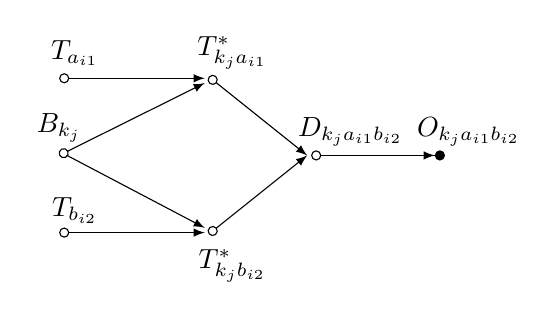
\begin{tikzpicture}

    % outcome
    \node at (3.5,1) {$O_{{k_{j}a_{i1}b_{i2}}}$};

    % difference
    \node at (2,1) {$D_{{k_{j}a_{i1}b_{i2}}}$};
    \draw[{Circle[open]}-{latex}{Circle}](1.5,0.7) to (3.2,0.7); 
    
    % "perceived" discriminal process for sub-unit
    \node at (0.5,2) {$T^{*}_{k_{j}a_{i1}}$};
    \draw[{Circle[open]}-{latex}](0.2,1.7) to (1.45,0.7); 

    % "true" discriminal process for sub-unit
    \node at (-1.5,2) {$T_{a_{i1}}$};
    \draw[{Circle[open]}-{latex}](-1.7,1.68) to (0.15,1.68); 
    
    % judges' biases
    \node at (-1.7,1.05) {$B_{k_{j}}$};
    \draw[{Circle[open]}-{latex}](-1.7,0.7) to (0.15,1.62); 
    \draw[-{latex}](-1.6,0.7) to (0.15,-0.22);
    
    % "perceived" discriminal process for sub-unit
    \node at (0.5,-0.7) {$T^{*}_{k_{j}b_{i2}}$};
    \draw[{Circle[open]}-{latex}](0.2,-0.3) to (1.45,0.7);     

    % "true" discriminal process for sub-unit
    \node at (-1.5,0) {$T_{b_{i2}}$};
    \draw[{Circle[open]}-{latex}](-1.7,-0.28) to (0.15,-0.28);     
    
\end{tikzpicture}

\end{document}
